\def\year{2019}\relax
%File: formatting-instruction.tex
\documentclass[letterpaper]{article} % DO NOT CHANGE THIS
\usepackage{aaai19}  % DO NOT CHANGE THIS
\usepackage{times}  % DO NOT CHANGE THIS
\usepackage{helvet} % DO NOT CHANGE THIS
\usepackage{courier}  % DO NOT CHANGE THIS
\usepackage[hyphens]{url}  % DO NOT CHANGE THIS
\usepackage{graphicx} % DO NOT CHANGE THIS
\urlstyle{rm} % DO NOT CHANGE THIS
\def\UrlFont{\rm}  % DO NOT CHANGE THIS
\usepackage{graphicx}  % DO NOT CHANGE THIS
\usepackage[labelfont=bf]{caption}
\frenchspacing  % DO NOT CHANGE THIS
\setlength{\pdfpagewidth}{8.5in}  % DO NOT CHANGE THIS
\setlength{\pdfpageheight}{11in}  % DO NOT CHANGE THIS

%PDF Info Is REQUIRED.
% For /Author, add all authors within the parentheses, separated by commas. No accents or commands.
% For /Title, add Title in Mixed Case. No accents or commands. Retain the parentheses.
 \pdfinfo{
/Title (Sentiment Analysis on Amazon Fine Food Review Dataset)
/Author (Xinyi Li, Hongzhi Liu, Sheng Wang, Siyu Zhang)
} %Leave this	
% /Title ()
% Put your actual complete title (no codes, scripts, shortcuts, or LaTeX commands) within the parentheses in mixed case
% Leave the space between \Title and the beginning parenthesis alone
% /Author ()
% Put your actual complete list of authors (no codes, scripts, shortcuts, or LaTeX commands) within the parentheses in mixed case. 
% Each author should be only by a comma. If the name contains accents, remove them. If there are any LaTeX commands, 
% remove them. 

% DISALLOWED PACKAGES
% \usepackage{authblk} -- This package is specifically forbidden
% \usepackage{balance} -- This package is specifically forbidden
% \usepackage{caption} -- This package is specifically forbidden
% \usepackage{color (if used in text)
% \usepackage{CJK} -- This package is specifically forbidden
% \usepackage{float} -- This package is specifically forbidden
% \usepackage{flushend} -- This package is specifically forbidden
% \usepackage{fontenc} -- This package is specifically forbidden
% \usepackage{fullpage} -- This package is specifically forbidden
% \usepackage{geometry} -- This package is specifically forbidden
% \usepackage{grffile} -- This package is specifically forbidden
% \usepackage{hyperref} -- This package is specifically forbidden
% \usepackage{navigator} -- This package is specifically forbidden
% (or any other package that embeds links such as navigator or hyperref)
% \indentfirst} -- This package is specifically forbidden
% \layout} -- This package is specifically forbidden
% \multicol} -- This package is specifically forbidden
% \nameref} -- This package is specifically forbidden
% \natbib} -- This package is specifically forbidden -- use the following workaround:
% \usepackage{savetrees} -- This package is specifically forbidden
% \usepackage{setspace} -- This package is specifically forbidden
% \usepackage{stfloats} -- This package is specifically forbidden
% \usepackage{tabu} -- This package is specifically forbidden
% \usepackage{titlesec} -- This package is specifically forbidden
% \usepackage{tocbibind} -- This package is specifically forbidden
% \usepackage{ulem} -- This package is specifically forbidden
% \usepackage{wrapfig} -- This package is specifically forbidden
% DISALLOWED COMMANDS
% \nocopyright -- Your paper will not be published if you use this command
% \addtolength -- This command may not be used
% \balance -- This command may not be used
% \baselinestretch -- Your paper will not be published if you use this command
% \clearpage -- No page breaks of any kind may be used for the final version of your paper
% \columnsep -- This command may not be used
% \newpage -- No page breaks of any kind may be used for the final version of your paper
% \pagebreak -- No page breaks of any kind may be used for the final version of your paperr
% \pagestyle -- This command may not be used
% \tiny -- This is not an acceptable font size.
% \vspace{- -- No negative value may be used in proximity of a caption, figure, table, section, subsection, subsubsection, or reference
% \vskip{- -- No negative value may be used to alter spacing above or below a caption, figure, table, section, subsection, subsubsection, or reference

\setcounter{secnumdepth}{2} %May be changed to 1 or 2 if section numbers are desired.

% The file aaai19.sty is the style file for AAAI Press 
% proceedings, working notes, and technical reports.
%
\setlength\titlebox{2.5in} % If your paper contains an overfull \vbox too high warning at the beginning of the document, use this
% command to correct it. You may not alter the value below 2.5 in
\title{Sentiment Analysis on Amazon Fine Food Review Dataset}
%Your title must be in mixed case, not sentence case. 
% That means all verbs (including short verbs like be, is, using,and go), 
% nouns, adverbs, adjectives should be capitalized, including both words in hyphenated terms, while
% articles, conjunctions, and prepositions are lower case unless they
% directly follow a colon or long dash
\author{Xinyi Li, Hongzhi Liu, Sheng Wang, Siyu Zhang\textsuperscript{\rm 1}\\ \\ % All authors must be in the same font size and format. Use \Large and \textbf to achieve this result when breaking a line
\textsuperscript{\rm 1}University of Wisconsin-Madison\\ %If you have multiple authors and multiple affiliations
% use superscripts in text and roman font to identify them. For example, Sunil Issar,\textsuperscript{\rm 2} J. Scott Penberthy\textsuperscript{\rm 3} George Ferguson,\textsuperscript{\rm 4} Hans Guesgen\textsuperscript{\rm 5}. Note that the comma should be placed BEFORE the superscript for optimum readability
%2275 East Bayshore Road, Suite 160\\
%Palo Alto, California 94303\\
%publications19@aaai.org % email address must be in roman text type, not monospace or sans serif
}
 \begin{document}

\maketitle

\begin{abstract}
In this project, we conducted a sentiment analysis for fine food reviews using natural language processing. A recurrent neural network was built to predict the user rating for fine food according to the comment. Model hyperparameters were selected according the cross validation analysis. Overfitting issue was discussed for this model. A precison/recall curve was plotted based on the model output. 

\end{abstract}


\section{Introduction}

Sentiment analysis is an automated process of understanding opinions from natural language. Nowadays countless reviews are available on internet, but almost all of them are unstructured data, making direct analysis difficult and time-consuming. Sentiment analysis can help address this issue by quantifying the information in unstructured data, thus the polarity hidden behind the texts can be extracted for further analysis. 

Recently, sentiment analysis has gained much popularity and has been used to resolve many practical issues, such as marketing analysis, customer service, etc. In this report, we apply sentiment analysis on Amazon fine food review dataset from Stanford Network Analysis Project (SNAP) which contains $568,454$ reviews from more than $200,000$ users to study customer behavior and predict the ratings. There are many methods to implement sentiment analysis when our goal is to predict the level of polarity of opinions (thus can be viewed as a classification problem), such as Logistic Regression, Support Vector Machine, Neural Network. Since the model needs to process language input, we chose Recurrent Neural Network(RNN) with embedding for this problem set.

\section{Feature Selection}

The data we use is Amazon fine food review dataset from SNAP. It contains $568,454$ reviews from more than $200,000$ users which are collected between Oct $1999$ and Oct $2012$. Each data instance consists of $10$ variables including product ID, user information, profile name of the user, number of users who found the review helpful(HelpfulnessNumerator), number of users who indicated whether they found the review helpful or not(HelpfulnessDenominator), rating, timestamp for the review, brief summary of the review, and plain text review. The statistics of major variables are shown in Table 1.




\begin{table}
\centering
\resizebox{.95\columnwidth}{!}{
\smallskip\begin{tabular}{l|l} 
\hline
Num. of Products               & 74258                \\ 
\hline
Num. of Users                  & 256059               \\ 
\hline
HelpfulnessNumerator Average   & 1.743817             \\ 
\hline
HelpfulnessDenominator Average & 2.22881              \\ 
\hline
Score Average                  & 4.183199             \\ 
\hline
Time                           & Oct 1999 - Oct 2012  \\
\hline
\end{tabular}
}
\caption{Summary for Variables in Amazon Fine Food Review}\smallskip
\label{table1}
\end{table}

Among all the features provided in the data set, we select HelpfulnessNumerator, HelpfulnessDenominator, summary of reviews and text review to predict the ratings of a given product by this user. Other variables are considered irrelevant here.


\begin{figure}[!h]
\centering
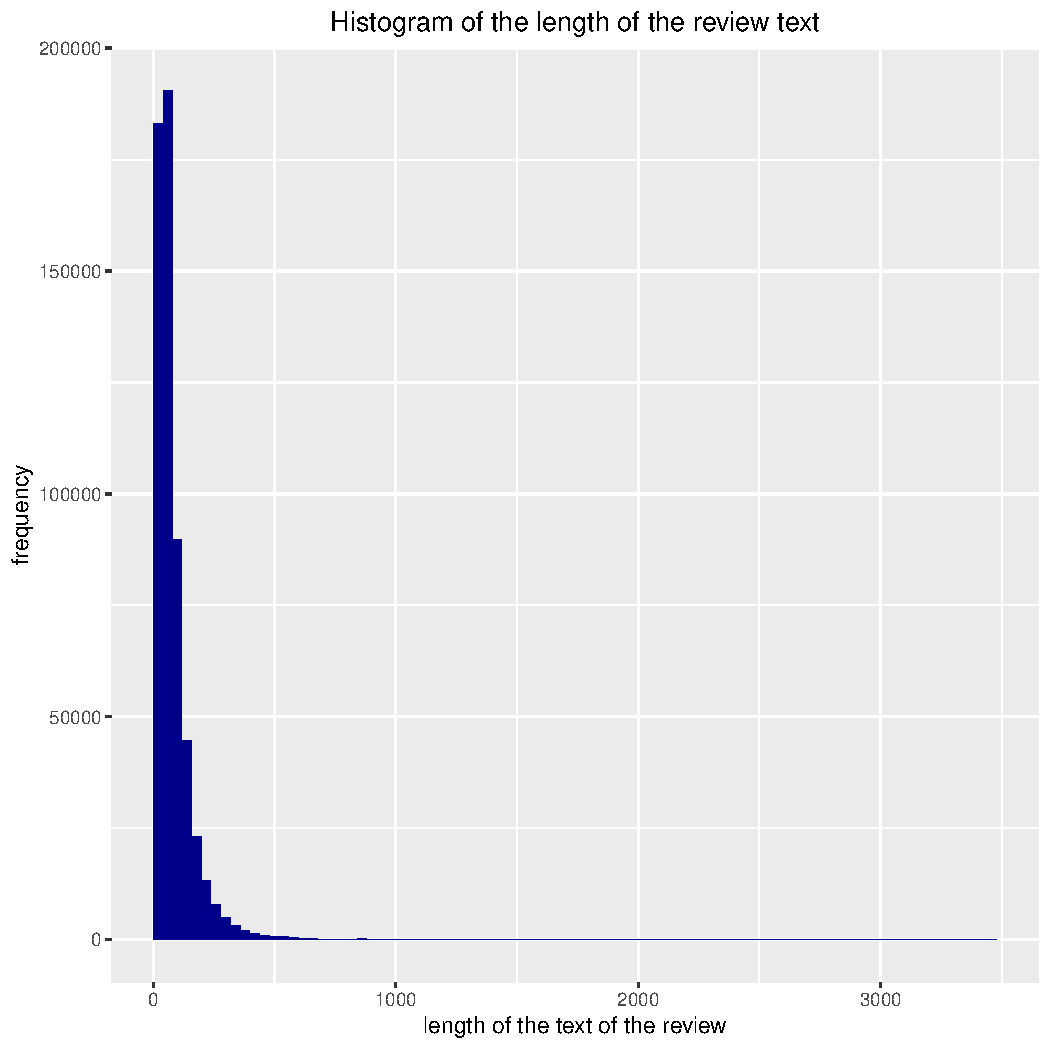
\includegraphics[height=7cm,width=0.9\columnwidth]{pics//plot_t_len.pdf} % Reduce the figure size so that it is slightly narrower than the column. Don't use precise values for figure width.This setup will avoid overfull boxes. 
\caption{Distribution of Length of the Reviews. X axis is the length of Review for each user, and y axis represents the frequency for each Review length.}
\label{Review Length}
\end{figure}

\begin{figure}[!h]
\centering
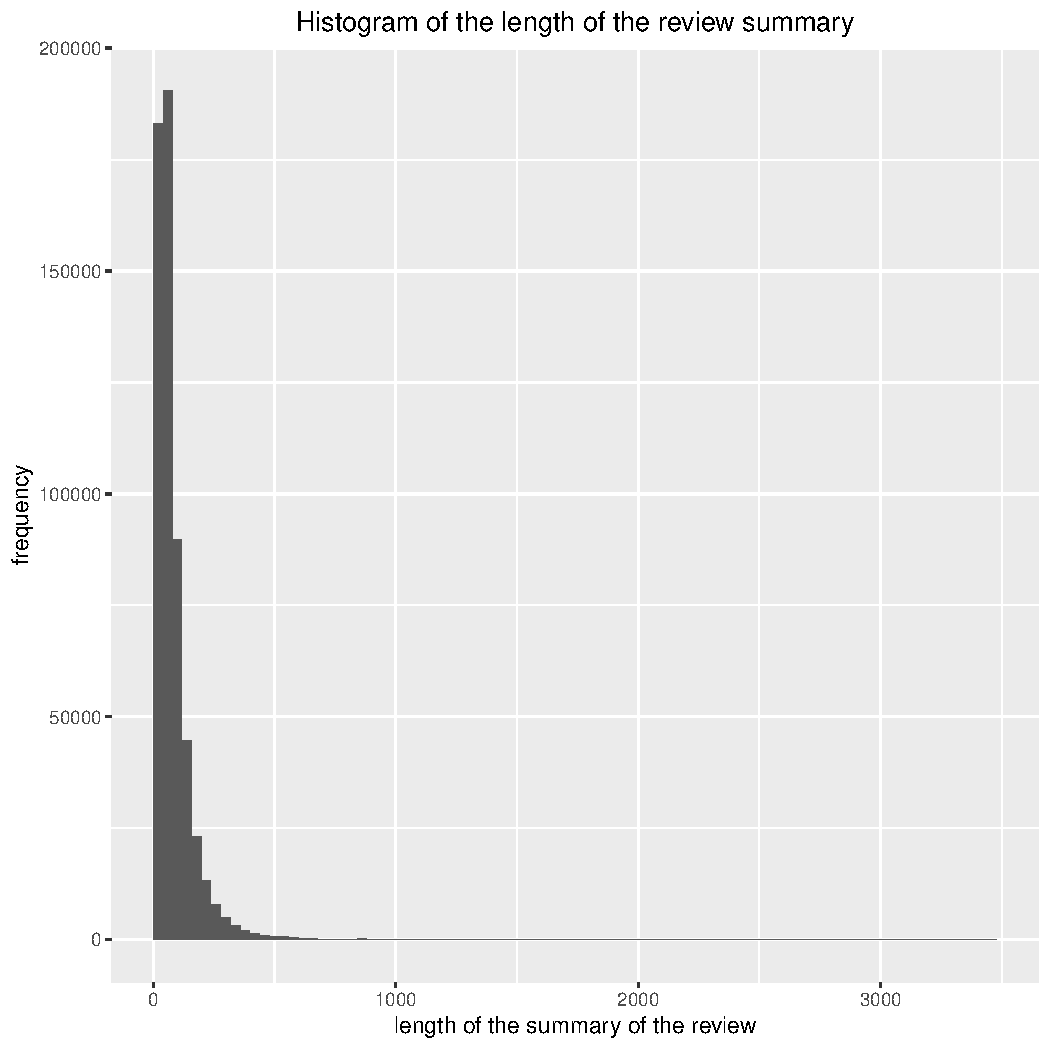
\includegraphics[height=7cm,width=0.9\columnwidth]{pics//plot_r_len.pdf} 
\caption{Distribution of Length of Summary. X axis is the length of variable Summary for each user, and y axis represents the frequency for each Summary length.}
\label{Summary Length}
\end{figure}

\begin{figure}[!h]
\centering
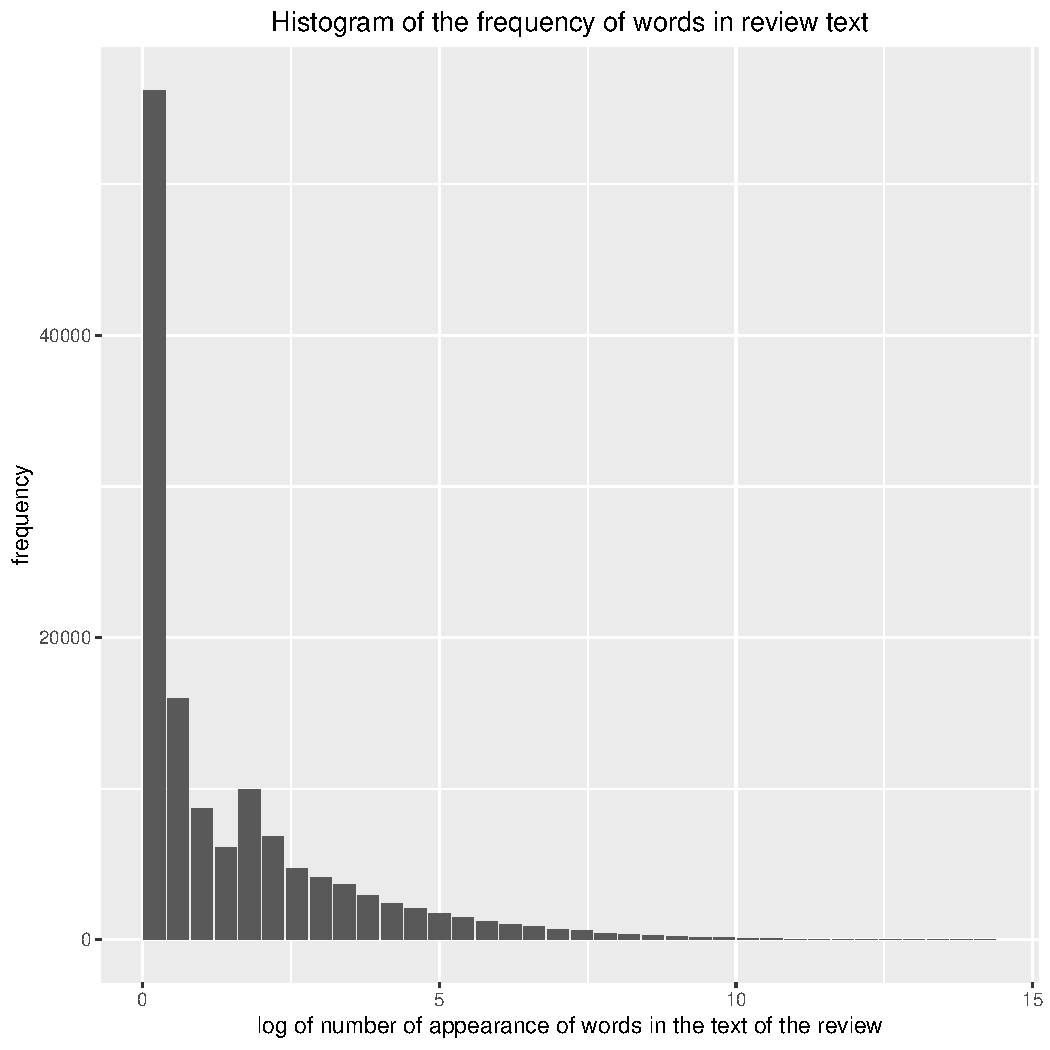
\includegraphics[height=7cm,width=0.9\columnwidth]{pics//plot_t_freq.pdf}  
\caption{Distribution of Word Frequency of Text in Review. We count the total number of appearance of each word in Review, and then take logarithm transformation to better view the distribution, and y axis denotes the frequency for each log of total appearances.}
\label{Review Frequency}
\end{figure}

\begin{figure}[!h]
\centering
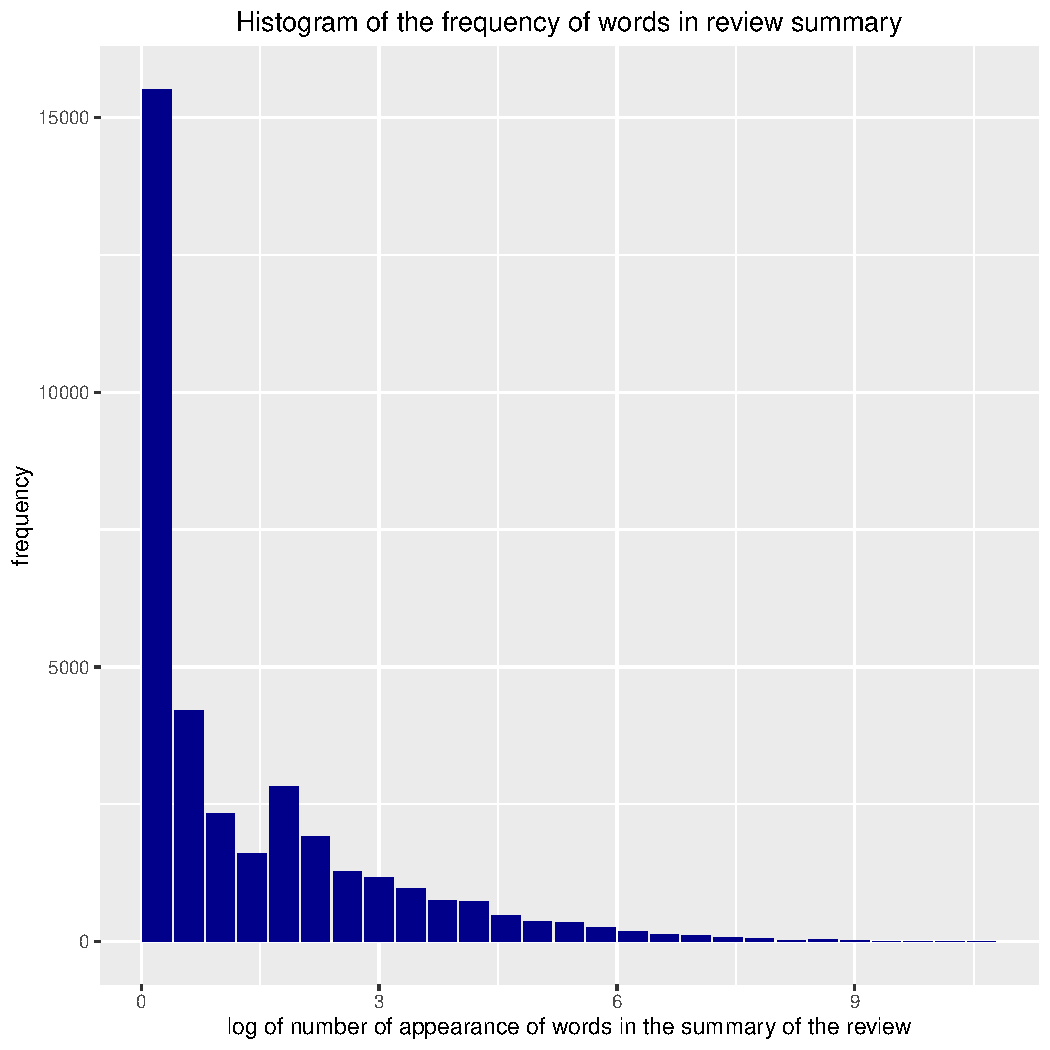
\includegraphics[height=7cm,width=0.9\columnwidth]{pics//plot_r_freq.pdf}  
\caption{Distribution of Word Frequency of Summary. We count the total number of appearance of each word in Summary, and then take logarithm transformation to better view the distribution, and y axis is the frequency for each log of total appearances.}
\label{Summary Frequency}
\end{figure}

But summary and reviews are not ready to be fed to the model directly, to structurize text information, we use a skip-gram model to do word-embeddings. The strength of this approach is that it projects texts to a lower-dimensional vector space while capturing the semantic similarity among words. Considering that the longest text reviews contains $3507$ words, but the majority of the text review length are below $300$ (see Fig.\ref{Review Length}), we can pad the review sequences at 300 to largely relieve computation challenge while still maintain accuracy. Similarly, as shown in Fig.\ref{Summary Length}, most of the review summaries has length under 50, so we choose to pad the summary sequence at 50. Another detail in feature extraction is that there are tens of thousands of words with extreme low frequency, as shown in Fig.\ref{Review Frequency} \& Fig.\ref{Summary Frequency}. Including these low-frequency words would offer us little benefit in text vectorization but lead in much computational burden. Hence, we only keep the $30,000$ most frequent words to effeciently extract text feature.

\begin{figure}[!h]
\centering
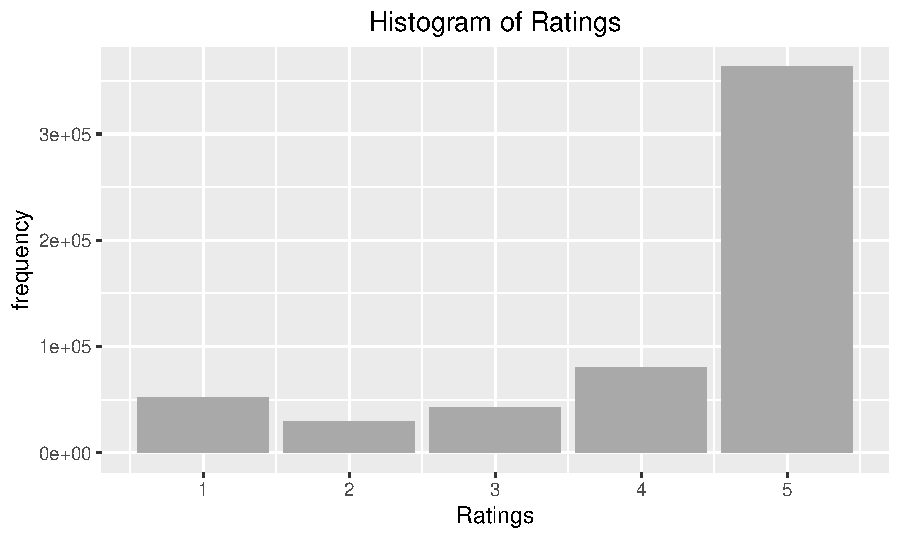
\includegraphics[width=0.9\columnwidth]{plot_rating.pdf}
\caption{Distribution of Ratings}
\label{Dstribution of Ratings.}
\end{figure}


By looking at the distribution of ratings shown in Fig.\ref{Dstribution of Ratings.}, we can see that it's highly skewed towards 5-star rating, which takes up to 63.9\% of all the ratings. Due to the unbalanced distribution of the rating, combined with the fact that the scores given by users can be quite subjective and uncertain, we merge ratings 1-3 as "bad" reviews, and ratings 4-5 as "good" reviews. In this way, the problem setting can better mimic the false feelings common in many people that the difference between 3-star and 4-star (from bad/neutral to good) is much bigger than that between 4 and 5(among good reviews) or between 2 and 3(among bad reviews). Now our prediction problem becomes a binary classification problem.

\section{Model Selection and Empirical Evaluation}
We built a model based on user review, brief summary of the review and the information whether the review is useful. The scheme of the model is shown in Fig.\ref{model}. Review and summary contains text information which needs to be processed. We first converted such text information to lower case and selected 30000 most common words for each as the library for one-hot encoding. Then all reviews and summaries were translated to sequences of one-hot vector according to preset library. Words which do not exit in the library were convert to vectors of 0. Before inputted into the model, sequences were padded to the same length. Review sequences were padded at length 300 and Summary sequences were padded at length 50. 

\begin{figure}[!h]
\centering
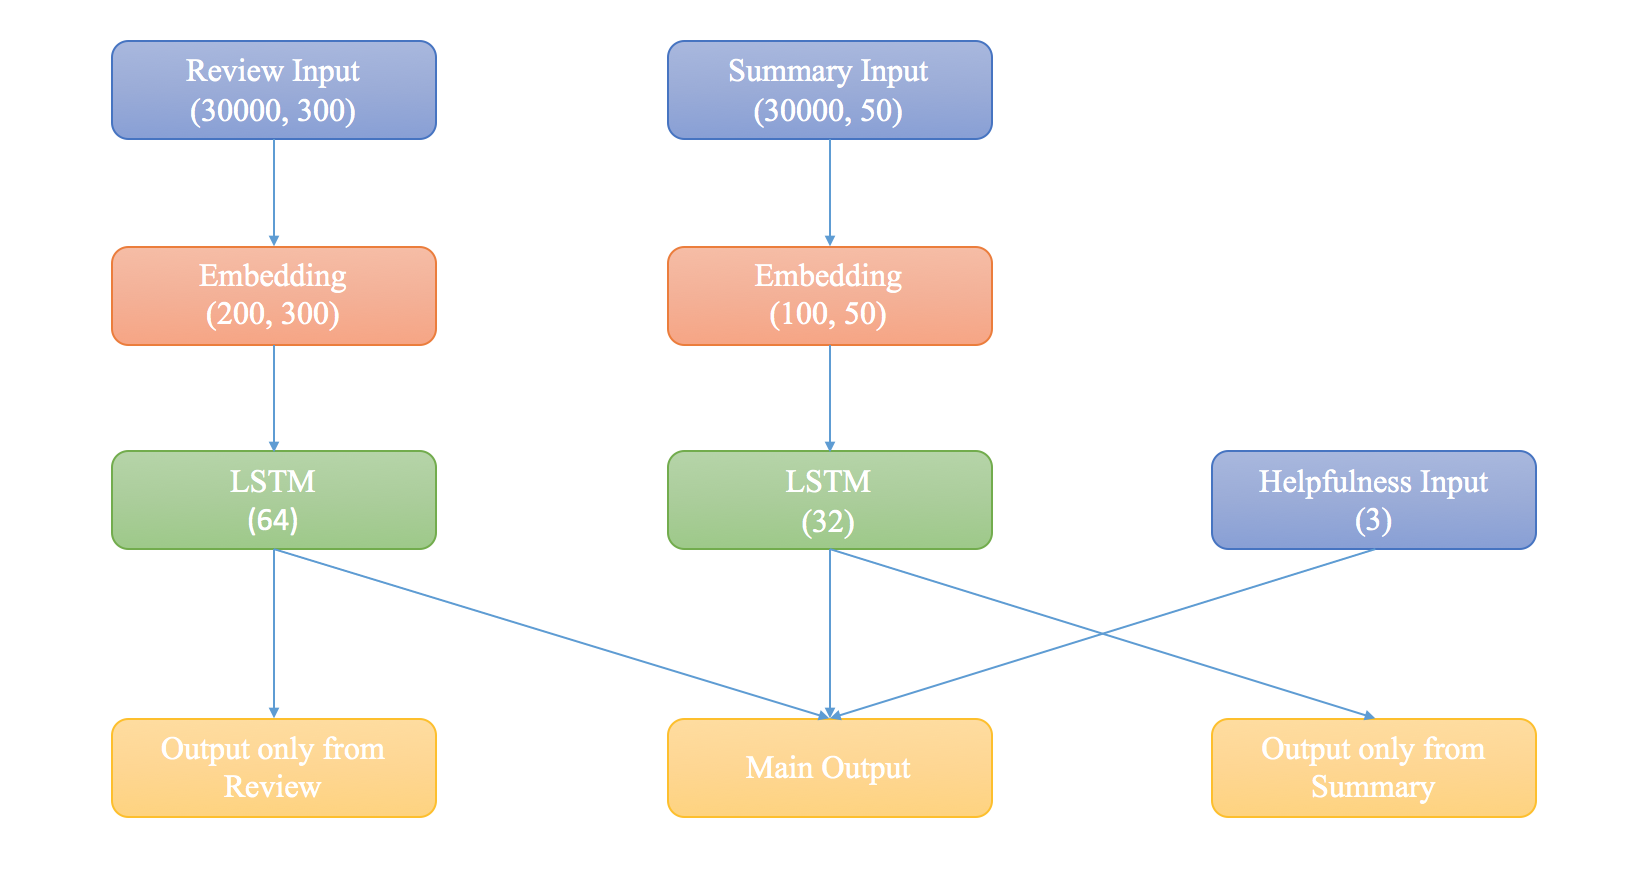
\includegraphics[height=6cm,width=1.0\columnwidth]{pics/structure_plot_2.png}
\caption{Structure Diagram of the Neural Net.}
\label{model}
\end{figure}

The preprocessed review sequences were inputted into an embedding layer and trained into sequences of vectors with 200 dimensions. The embedded sequences were used as the input of the LSTM layer with 64 hidden units. 20\% units were dropped out for inputs and recurrent state. The output of this LSTM layer were trained to a binary output using sigmoid function as the activation function and binary crossentropy as the loss function. 

The same training model was applied on summary data. Since summary data contains less information. Only 32 hidden units of LSTM layer were employed here. A binary output was produced based only on summary data.
In addition, the outputs of both LSTM layers were combined along with "helpfulness" data as the input of a third perceptron. The "helpfulness" data are processed from number of users who found the review helpful(HelpfulnessNumerator) and number of users who indicated whether they found the review helpful or not(HelpfulnessDenominator). In addition to the above two features, the ratio between them are calculated as the third feature for this "helpfulness" data. The output of this third perceptron was used as the main output of this model.

In summary, three outputs were produced from this model based on review, summary of the review and the "helpfulness" information. One of the outputs is the prediction only based on the review data. Another is only based on the summary data. The main output of this model learns information from all input data. 

Most hyperparameters of the model are selected from detailed feature analysis and previous experience of natural language processing. The model was fitted on the training data using stochastic learning. To better utilize the parallel processing power of GPUs, we selected batch size as 500. The cost of training each instance using GPU with respect to the batch size is plotted in Fig.\ref{batch_size}. Considering the total size of the dataset(568,454), 500 is also an appropriate selection for batch size. Adam was selected as optimizer with learning rate 0.001.

\begin{figure}[!h]
\centering
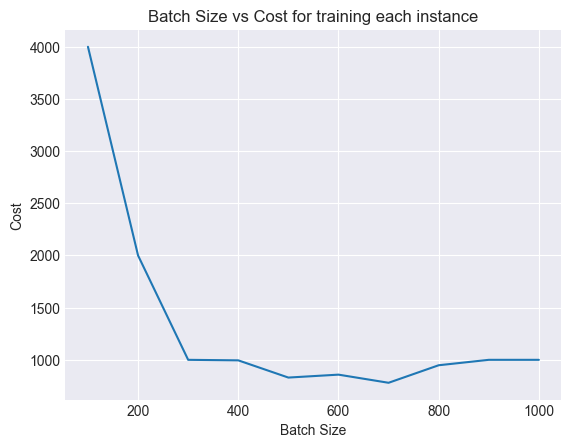
\includegraphics[width=0.9\columnwidth]{pics/pr_batch.png}
\caption{Batch Size vs Cost for Training Each Instance.}
\label{batch_size}
\end{figure}

 To avoid underfitting, we also added another LSTM layer for each recurrent network in this model and checked the corresponding performance. Comparison of the accuracy of 1-layer-LSTM model and 2-layer-LSTM model are listed in Fig.\ref{predAcc}.

\begin{figure}[!h]
\centering
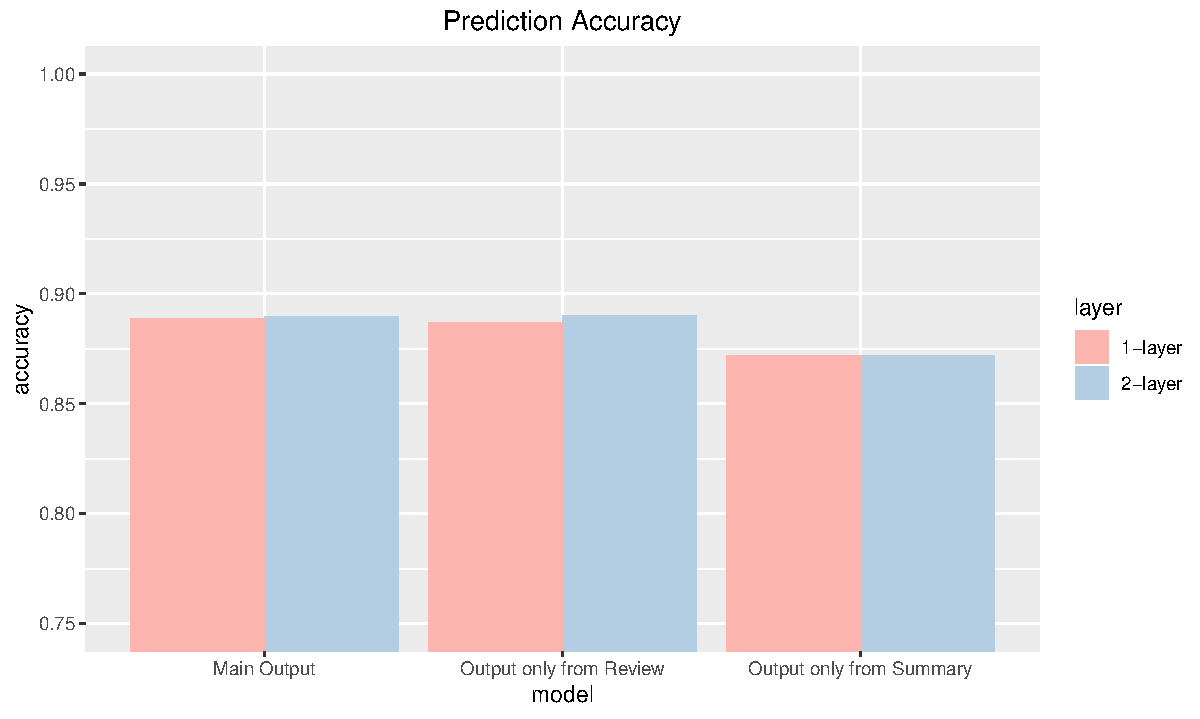
\includegraphics[width=1.0\columnwidth]{plot_acc.pdf}
\caption{Prediction Accuracy of Two Candidate Models. We compare the prediction accuracy for 1-layer-LSTM model and 2-layer-LSTM model, and we measure the differences based on three kinds of output: main output, output only from Review, and output only from Summary. }
\label{predAcc}
\end{figure}


\begin{figure}[!h]
\centering
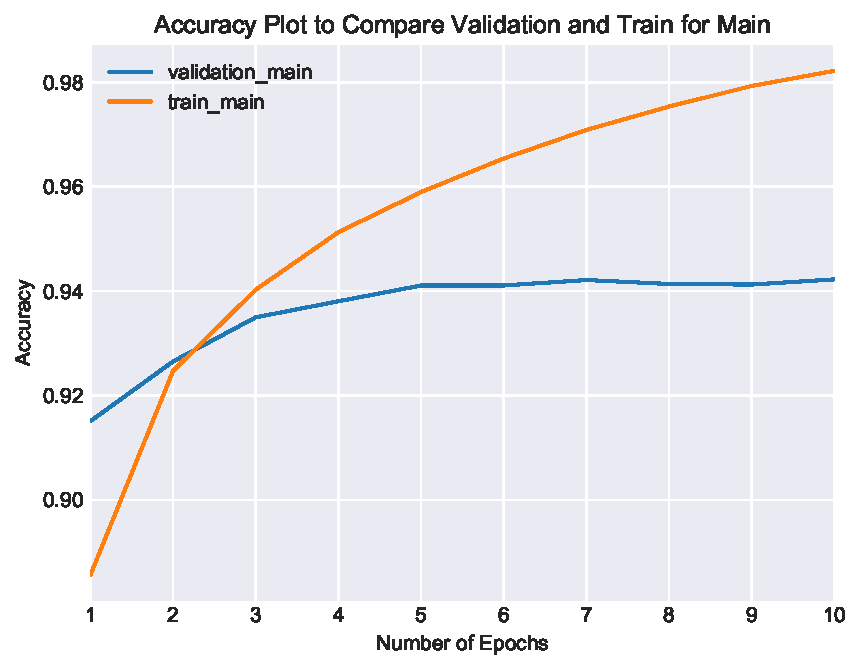
\includegraphics[height=7cm,width=0.9\columnwidth]{train_val_main.pdf}  
\caption{Validation and Train Accuracy for Main. The orange line represents train accuracy, and the blue line denotes the validation accuracy.}
\label{epochs}
\end{figure}


For this comparison, we randomly selected 100000 data to run cross validation. Number of epochs were chose as 2. From Fig.\ref{predAcc}, we can observe that adding a LSTM layer does not significantly increase the fitting accuracy. For simplicity, we only employ 1 LSTM layer in this model.

We also calculated accuracy curve for main output with respect to number of epochs as plotted in Fig.\ref{epochs}. In this simulation, we utilize all the data from the dataset. 80\% data were chosen as traing data and the remianing were used as validation data.








In this plot, accuracy of validation set reaches a plateau when number of epochs is 5. However, the accuracy of the training set still increases. It indicates that when the number of epochs is larger than 5, model overfits the data. Although they are not plotted here, accuracy of outputs from only review data and only summary data have the same behavior. 

\section{Data Analysis}

In this section, we further analyze the performance of the three in previous sections: one based only on Text Reviews, another based only on Summary, and a third output uses all the information in Text Reviews, Summary and  the information whether the review is useful. 

We first look at the accuracy of the three models on the test set shown in Fig.\ref{1}. When the number of epochs is fixed at 5, the accuracy of the main output outperforms the other two. This comparison indicates that there exists useful information hidden in the HelpfulnessNumerator and HelpfulnessDenominator.

\begin{figure}[!h]
\centering
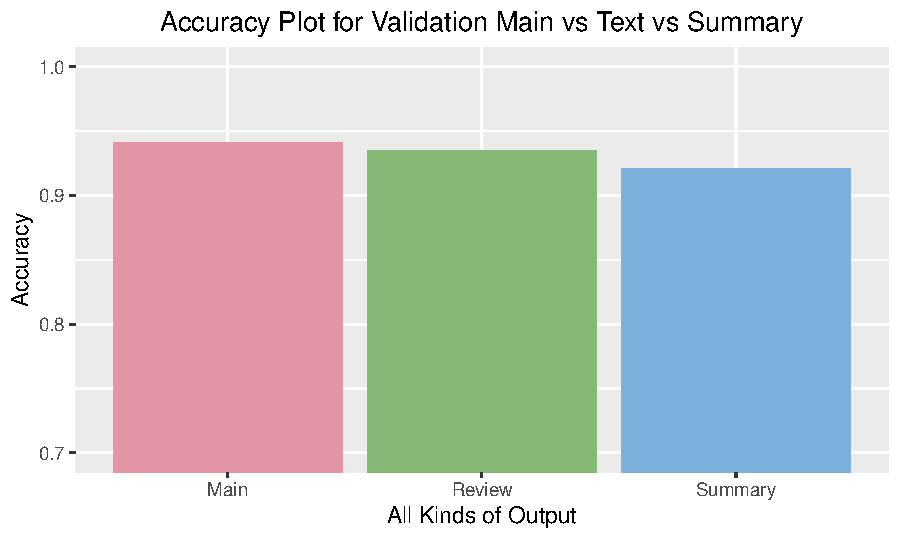
\includegraphics[height=6cm,width=0.9\columnwidth]{plot_val_acc.pdf}  
\caption{Training Accuracy Plot for Main vs Review vs Summary. We Compare the training accuracy using three different inputs: Main, Review, and Summary. The blue line represents Main output, the orange line denotes Review output, and green line corresponds to Summary output.}
\label{1}
\end{figure}


\begin{figure}[!h]
\centering
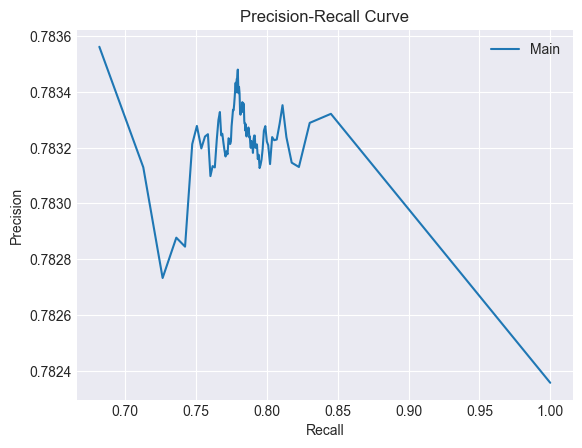
\includegraphics[height=7cm,width=0.9\columnwidth]{pr_curve.png}  
\caption{Precision/Recall Curve. This curve is based on the Main output.}
\label{3}
\end{figure}

Because of the unbalanced nature of this dataset, the accuracy measure can sometimes be misleading. Here we also include a Precision-Recall Curve, which can not only give us the full picture of the performance of the model as the threshold changes, but also are robust to the skewness of classes. From Fig.\ref{3} we can see that the area under this PR curve is close to 1, indicating that our model is well-trained and offer much predictability.

The accuracy of the main output reaches $94\%$.  This high accuracy is still informative in spite of the high skewness of the data, because the ratio of the "good" reviews accounts for $78\%$, which is much lower than our $94\%$ accuracy (which means that the a "naive" classifier that classifies all data points as positive can only reach a $78\%$ accuracy).

It is also worth mentioning that our method is efficient when working with this huge dataset($568,454$ reviews) containing sequence data and dealing with the natural language processing problem. The entire process to train all the five epochs takes only 32 minutes using current available GPUs.   

\section{Conclusion}
In this project, we developed an efficient RNN network to conduct sentiment analysis based on user reviews. In the future, we hope to refine the model to be able to predict the 5$\sim$scale user ratings. This may require a more complicated model and more careful parameter selection. We are also looking forward to adding more meaningful features like the length of review to our model to enhance the performance. 

\end{document}
